\begin{minipage}{0.265\textwidth}
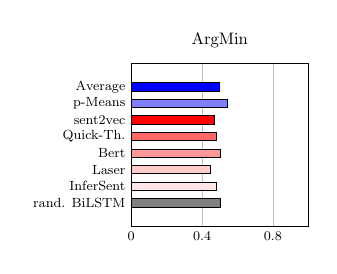
\begin{tikzpicture}[scale=0.75,every node/.style={scale=0.8}]

  	\begin{axis}[
		title=ArgMin,
 	   	xbar stacked,
		bar width=4pt,
		enlarge y limits=0.2,
    		symbolic y coords={rand. BiLSTM,InferSent,Laser,Bert,Quick-Th.,sent2vec,p-Means,Average},
		xmin=0,xmax=1,
  		xmajorgrids,
		tickwidth=0pt,
		xtick distance=0.40,
  		ytick=data,
		scale only axis=true,
  		width=3cm,height=2.75cm,
		tick label style={font=\footnotesize}
  	]

		% Average
  		\addplot[blue,fill,draw=black] coordinates
  			{(0.500,Average) (0.00,p-Means) (0.00,sent2vec) (0.00,Quick-Th.) (0.00,Bert) (0.00,Laser) (0.00,InferSent) (0.00,rand. BiLSTM)};
		% p-Means
		\addplot[blue!50,fill,draw=black] coordinates
			{(0.00,Average) (0.541,p-Means) (0.00,sent2vec) (0.00,Quick-Th.) (0.00,Bert) (0.00,Laser) (0.00,InferSent) (0.00,rand. BiLSTM)};

		% sent2vec
		\addplot[red,fill,draw=black] coordinates 
			{(0.00,Average) (0.00,p-Means) (0.472,sent2vec) (0.00,Quick-Th.) (0.00,Bert) (0.00,Laser) (0.00,InferSent) (0.00,rand. BiLSTM)};
		% Quick-Th.
		\addplot[red!60,fill,draw=black] coordinates
			{(0.00,Average) (0.00,p-Means) (0.00,sent2vec) (0.482,Quick-Th.) (0.00,Bert) (0.00,Laser) (0.00,InferSent) (0.00,rand. BiLSTM)};
		% Bert
		\addplot[red!40,fill,draw=black] coordinates
			{(0.00,Average) (0.00,p-Means) (0.00,sent2vec) (0.00,Quick-Th.) (0.502,Bert) (0.00,Laser) (0.00,InferSent) (0.00,rand. BiLSTM)};
		% Laser
		\addplot[red!20,fill,draw=black] coordinates
			{(0.00,Average) (0.00,p-Means) (0.00,sent2vec) (0.00,Quick-Th.) (0.00,Bert) (0.449,Laser) (0.00,InferSent) (0.00,rand. BiLSTM)};
		% InferSentent
		\addplot[red!10,fill,draw=black] coordinates
			{(0.00,Average) (0.00,p-Means) (0.00,sent2vec) (0.00,Quick-Th.) (0.00,Bert) (0.00,Laser) (0.479,InferSent) (0.00,rand. BiLSTM)};

		% rand lstm
		\addplot[gray,fill,draw=black] coordinates 
			{(0.00,Average) (0.00,p-Means) (0.00,sent2vec) (0.00,Quick-Th.) (0.00,Bert) (0.00,Laser) (0.00,InferSent) (0.506,rand. BiLSTM)};

  	\end{axis}

\end{tikzpicture}
\end{minipage}
\hspace*{16mm}
\begin{minipage}{0.25\textwidth}
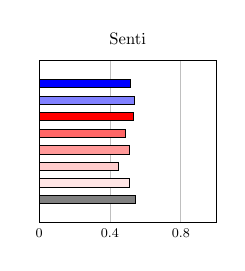
\begin{tikzpicture}[scale=0.75,every node/.style={scale=0.8}]

  	\begin{axis}[
		title=Senti,
   	 	xbar stacked,
		bar width=4pt,
		enlarge y limits=0.2,
	    	symbolic y coords={rand. BiLSTM,InferSent,Laser,Bert,Quick-Th.,sent2vec,p-Means,Average},
		xmin=0,xmax=1,
  		xmajorgrids,
		tickwidth=0pt,
		xtick distance=0.40,
  		ytick=data,
		yticklabels={,,},
		scale only axis=true,
  		width=3cm,height=2.75cm,
		tick label style={font=\footnotesize}
  	]

		% Average
  		\addplot[blue,fill,draw=black] coordinates
  			{(0.514,Average) (0.00,p-Means) (0.00,sent2vec) (0.00,Quick-Th.) (0.00,Bert) (0.00,Laser) (0.00,InferSent) (0.00,rand. BiLSTM)};
		% p-Means
		\addplot[blue!50,fill,draw=black] coordinates
			{(0.00,Average) (0.539,p-Means) (0.00,sent2vec) (0.00,Quick-Th.) (0.00,Bert) (0.00,Laser) (0.00,InferSent) (0.00,rand. BiLSTM)};

		% sent2vec
		\addplot[red,fill,draw=black] coordinates 
			{(0.00,Average) (0.00,p-Means) (0.531,sent2vec) (0.00,Quick-Th.) (0.00,Bert) (0.00,Laser) (0.00,InferSent) (0.00,rand. BiLSTM)};
		% Quick-Th.
		\addplot[red!60,fill,draw=black] coordinates
			{(0.00,Average) (0.00,p-Means) (0.00,sent2vec) (0.488,Quick-Th.) (0.00,Bert) (0.00,Laser) (0.00,InferSent) (0.00,rand. BiLSTM)};
		% Bert
		\addplot[red!40,fill,draw=black] coordinates
			{(0.00,Average) (0.00,p-Means) (0.00,sent2vec) (0.00,Quick-Th.) (0.511,Bert) (0.00,Laser) (0.00,InferSent) (0.00,rand. BiLSTM)};
		% Laser
		\addplot[red!20,fill,draw=black] coordinates
			{(0.00,Average) (0.00,p-Means) (0.00,sent2vec) (0.00,Quick-Th.) (0.00,Bert) (0.450,Laser) (0.00,InferSent) (0.00,rand. BiLSTM)};
		% InferSentent
		\addplot[red!10,fill,draw=black] coordinates
			{(0.00,Average) (0.00,p-Means) (0.00,sent2vec) (0.00,Quick-Th.) (0.00,Bert) (0.00,Laser) (0.510,InferSent) (0.00,rand. BiLSTM)};

		% rand lstm
		\addplot[gray,fill,draw=black] coordinates 
			{(0.00,Average) (0.00,p-Means) (0.00,sent2vec) (0.00,Quick-Th.) (0.00,Bert) (0.00,Laser) (0.00,InferSent) (0.546,rand. BiLSTM)};

  	\end{axis}

\end{tikzpicture}
\end{minipage}
\hfill
\begin{minipage}{0.25\textwidth}
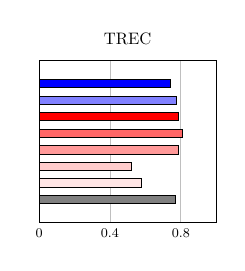
\begin{tikzpicture}[scale=0.75,every node/.style={scale=0.8}]

  	\begin{axis}[
		title=TREC,
 	   	xbar stacked,
		bar width=4pt,
		enlarge y limits=0.2,
    		symbolic y coords={rand. BiLSTM,InferSent,Laser,Bert,Quick-Th.,sent2vec,p-Means,Average},
		xmin=0,xmax=1,
  		xmajorgrids,
		tickwidth=0pt,
		xtick distance=0.40,
  		ytick=data,
		yticklabels={,,},
		scale only axis=true,
  		width=3cm,height=2.75cm,
		tick label style={font=\footnotesize}
  	]

		% Average
  		\addplot[blue,fill,draw=black] coordinates
  			{(0.739,Average) (0.00,p-Means) (0.00,sent2vec) (0.00,Quick-Th.) (0.00,Bert) (0.00,Laser) (0.00,InferSent) (0.00,rand. BiLSTM)};
		% p-Means
		\addplot[blue!50,fill,draw=black] coordinates
			{(0.00,Average) (0.774,p-Means) (0.00,sent2vec) (0.00,Quick-Th.) (0.00,Bert) (0.00,Laser) (0.00,InferSent) (0.00,rand. BiLSTM)};

		% sent2vec
		\addplot[red,fill,draw=black] coordinates 
			{(0.00,Average) (0.00,p-Means) (0.787,sent2vec) (0.00,Quick-Th.) (0.00,Bert) (0.00,Laser) (0.00,InferSent) (0.00,rand. BiLSTM)};
		% Quick-Th.
		\addplot[red!60,fill,draw=black] coordinates
			{(0.00,Average) (0.00,p-Means) (0.00,sent2vec) (0.811,Quick-Th.) (0.00,Bert) (0.00,Laser) (0.00,InferSent) (0.00,rand. BiLSTM)};
		% Bert
		\addplot[red!40,fill,draw=black] coordinates
			{(0.00,Average) (0.00,p-Means) (0.00,sent2vec) (0.00,Quick-Th.) (0.784,Bert) (0.00,Laser) (0.00,InferSent) (0.00,rand. BiLSTM)};
		% Laser
		\addplot[red!20,fill,draw=black] coordinates
			{(0.00,Average) (0.00,p-Means) (0.00,sent2vec) (0.00,Quick-Th.) (0.00,Bert) (0.523,Laser) (0.00,InferSent) (0.00,rand. BiLSTM)};
		% InferSentent
		\addplot[red!10,fill,draw=black] coordinates
			{(0.00,Average) (0.00,p-Means) (0.00,sent2vec) (0.00,Quick-Th.) (0.00,Bert) (0.00,Laser) (0.578,InferSent) (0.00,rand. BiLSTM)};

		% rand lstm
		\addplot[gray,fill,draw=black] coordinates 
			{(0.00,Average) (0.00,p-Means) (0.00,sent2vec) (0.00,Quick-Th.) (0.00,Bert) (0.00,Laser) (0.00,InferSent) (0.770,rand. BiLSTM)};

  	\end{axis}

\end{tikzpicture}
\end{minipage}
%\hfill
%\begin{minipage}{0.1\textwidth}
%\begin{tikzpicture}
%
%  	\begin{axis}[
% 	   	xbar stacked,
%		bar width=4pt,
%		enlarge y limits=0.2,
%    		symbolic y coords={rand. BiLSTM,InferSent,Laser,Bert,Quick-Th.,sent2vec,p-Means,Average},
%		xmin=0,xmax=1,
%  		xmajorgrids,
%		tickwidth=0pt,
%		xtick distance=0.40,
%  		ytick=data,
%		yticklabels={,,},
%		scale only axis=true,
%  		width=1.3cm,height=2cm,
%		tick label style={font=\tiny}
%  	]
%
%		% Average
%  		\addplot[blue,fill,draw=black] coordinates
%  			{(0.856,Average) (0.00,p-Means) (0.00,sent2vec) (0.00,Quick-Th.) (0.00,Bert) (0.00,Laser) (0.00,InferSent) (0.00,rand. BiLSTM)};
%		% p-Means
%		\addplot[blue!50,fill,draw=black] coordinates
%			{(0.00,Average) (0.848,p-Means) (0.00,sent2vec) (0.00,Quick-Th.) (0.00,Bert) (0.00,Laser) (0.00,InferSent) (0.00,rand. BiLSTM)};
%
%		% sent2vec
%		\addplot[red,fill,draw=black] coordinates 
%			{(0.00,Average) (0.00,p-Means) (0.807,sent2vec) (0.00,Quick-Th.) (0.00,Bert) (0.00,Laser) (0.00,InferSent) (0.00,rand. BiLSTM)};
%		% Quick-Th.
%		\addplot[red!60,fill,draw=black] coordinates
%			{(0.00,Average) (0.00,p-Means) (0.00,sent2vec) (0.794,Quick-Th.) (0.00,Bert) (0.00,Laser) (0.00,InferSent) (0.00,rand. BiLSTM)};
%		% Bert
%		\addplot[red!40,fill,draw=black] coordinates
%			{(0.00,Average) (0.00,p-Means) (0.00,sent2vec) (0.00,Quick-Th.) (0.842,Bert) (0.00,Laser) (0.00,InferSent) (0.00,rand. BiLSTM)};
%		% Laser
%		\addplot[red!20,fill,draw=black] coordinates
%			{(0.00,Average) (0.00,p-Means) (0.00,sent2vec) (0.00,Quick-Th.) (0.00,Bert) (0.791,Laser) (0.00,InferSent) (0.00,rand. BiLSTM)};
%		% InferSentent
%		\addplot[red!20,fill,draw=black] coordinates
%			{(0.00,Average) (0.00,p-Means) (0.00,sent2vec) (0.00,Quick-Th.) (0.00,Bert) (0.00,Laser) (0.850,InferSent) (0.00,rand. BiLSTM)};
%
%		% rand lstm
%		\addplot[gray,fill,draw=black] coordinates 
%			{(0.00,Average) (0.00,p-Means) (0.00,sent2vec) (0.00,Quick-Th.) (0.00,Bert) (0.00,Laser) (0.00,InferSent) (0.853,rand. BiLSTM)};
%
%  	\end{axis}
%
%\end{tikzpicture}
%\end{minipage}
%\hfill
%\begin{minipage}{0.1\textwidth}
%\begin{tikzpicture}
%
%  	\begin{axis}[
%   	 	xbar stacked,
%		bar width=4pt,
%		enlarge y limits=0.2,
%	    	symbolic y coords={rand. BiLSTM,InferSent,Laser,Bert,Quick-Th.,sent2vec,p-Means,Average},
%		xmin=0,xmax=1,
%  		xmajorgrids,
%		tickwidth=0pt,
%		xtick distance=0.40,
%  		ytick=data,
%		yticklabels={,,},
%		scale only axis=true,
%  		width=1.3cm,height=2cm,
%		tick label style={font=\tiny}
%  	]
%
%		% Average
%  		\addplot[blue,fill,draw=black] coordinates
%  			{(0.00,Average) (0.00,p-Means) (0.00,sent2vec) (0.00,Quick-Th.) (0.00,Bert) (0.00,Laser) (0.00,InferSent) (0.00,rand. BiLSTM)};
%		% p-Means
%		\addplot[blue!50,fill,draw=black] coordinates
%			{(0.00,Average) (0.00,p-Means) (0.00,sent2vec) (0.00,Quick-Th.) (0.00,Bert) (0.00,Laser) (0.00,InferSent) (0.00,rand. BiLSTM)};
%
%		% sent2vec
%		\addplot[red,fill,draw=black] coordinates 
%			{(0.00,Average) (0.00,p-Means) (0.00,sent2vec) (0.00,Quick-Th.) (0.00,Bert) (0.00,Laser) (0.00,InferSent) (0.00,rand. BiLSTM)};
%		% Quick-Th.
%		\addplot[red!60,fill,draw=black] coordinates
%			{(0.00,Average) (0.00,p-Means) (0.00,sent2vec) (0.00,Quick-Th.) (0.00,Bert) (0.00,Laser) (0.00,InferSent) (0.00,rand. BiLSTM)};
%		% Bert
%		\addplot[red!40,fill,draw=black] coordinates
%			{(0.00,Average) (0.00,p-Means) (0.00,sent2vec) (0.00,Quick-Th.) (0.00,Bert) (0.00,Laser) (0.00,InferSent) (0.00,rand. BiLSTM)};
%		% Laser
%		\addplot[red!20,fill,draw=black] coordinates
%			{(0.00,Average) (0.00,p-Means) (0.00,sent2vec) (0.00,Quick-Th.) (0.00,Bert) (0.00,Laser) (0.00,InferSent) (0.00,rand. BiLSTM)};
%		% InferSentent
%		\addplot[red!20,fill,draw=black] coordinates
%			{(0.00,Average) (0.00,p-Means) (0.00,sent2vec) (0.00,Quick-Th.) (0.00,Bert) (0.00,Laser) (0.00,InferSent) (0.00,rand. BiLSTM)};
%
%		% rand lstm
%		\addplot[gray,fill,draw=black] coordinates 
%			{(0.00,Average) (0.00,p-Means) (0.00,sent2vec) (0.00,Quick-Th.) (0.00,Bert) (0.00,Laser) (0.00,InferSent) (0.00,rand. BiLSTM)};
%
%  	\end{axis}
%
%\end{tikzpicture}
%\end{minipage}
%\hfill
%\begin{minipage}{0.1\textwidth}
%\begin{center}
%\textit{n.\,a.}
%\end{center}
%\end{minipage}
%\hfill
%\begin{minipage}{0.1\textwidth}
%\begin{center}
%\textit{n.\,a.}
%\end{center}
%\end{minipage}
%\hfill
%\begin{minipage}{0.1\textwidth}
%\begin{center}
%\textit{n.\,a.}
%\end{center}
%\end{minipage}